\chapter{Descripción de la aplicación web}
\label{chap:descripcion_aplicacion}

\lettrine{L}{os} capítulos precedentes han establecido el marco teórico que sustenta este proyecto: los fundamentos del modelado dimensional, los procesos ETL y las arquitecturas de visualización analítica. 

El resultado del proyecto es un cuadro de mando analítico accesible desde el navegador, cuyo usuario objetivo es el \textbf{técnico o inspector de la administración educativa autonómica} responsable de la distribución de recursos entre centros. La herramienta le permite responder a dos preguntas fundamentales de forma secuencial: en primer lugar, \textit{qué centros requieren mayor atención o dotación de recursos} en el conjunto de la comunidad autónoma; y en segundo lugar, \textit{por qué} un centro concreto presenta el índice de riesgo que presenta, desagregando las causas académicas, socioeconómicas y curriculares que lo explican.

Para dar respuesta a estas dos preguntas, la interfaz se estructura en dos vistas complementarias que comparten los mismos indicadores de alerta pero los miden a distinta escala. La \textbf{vista Macro} opera a escala autonómica: sus KPI cuentan el número de \textit{centros} que superan la mediana autonómica en cada métrica de riesgo. La \textbf{vista Micro} opera a escala de centro: sus KPI cuentan el número de \textit{alumnos} de los centros seleccionados que presentan cada factor de riesgo. El flujo natural de uso consiste en identificar centros prioritarios en la vista Macro y, a continuación, realizar un \textit{drilldown} hacia la vista Micro para diagnosticar las causas concretas del riesgo en esos centros, fundamentando así la decisión de asignación de recursos con evidencia objetiva.

% =========================================================================
\section{Flujo de acceso y autenticación}

\begin{figure}[htbp]
    \centering
    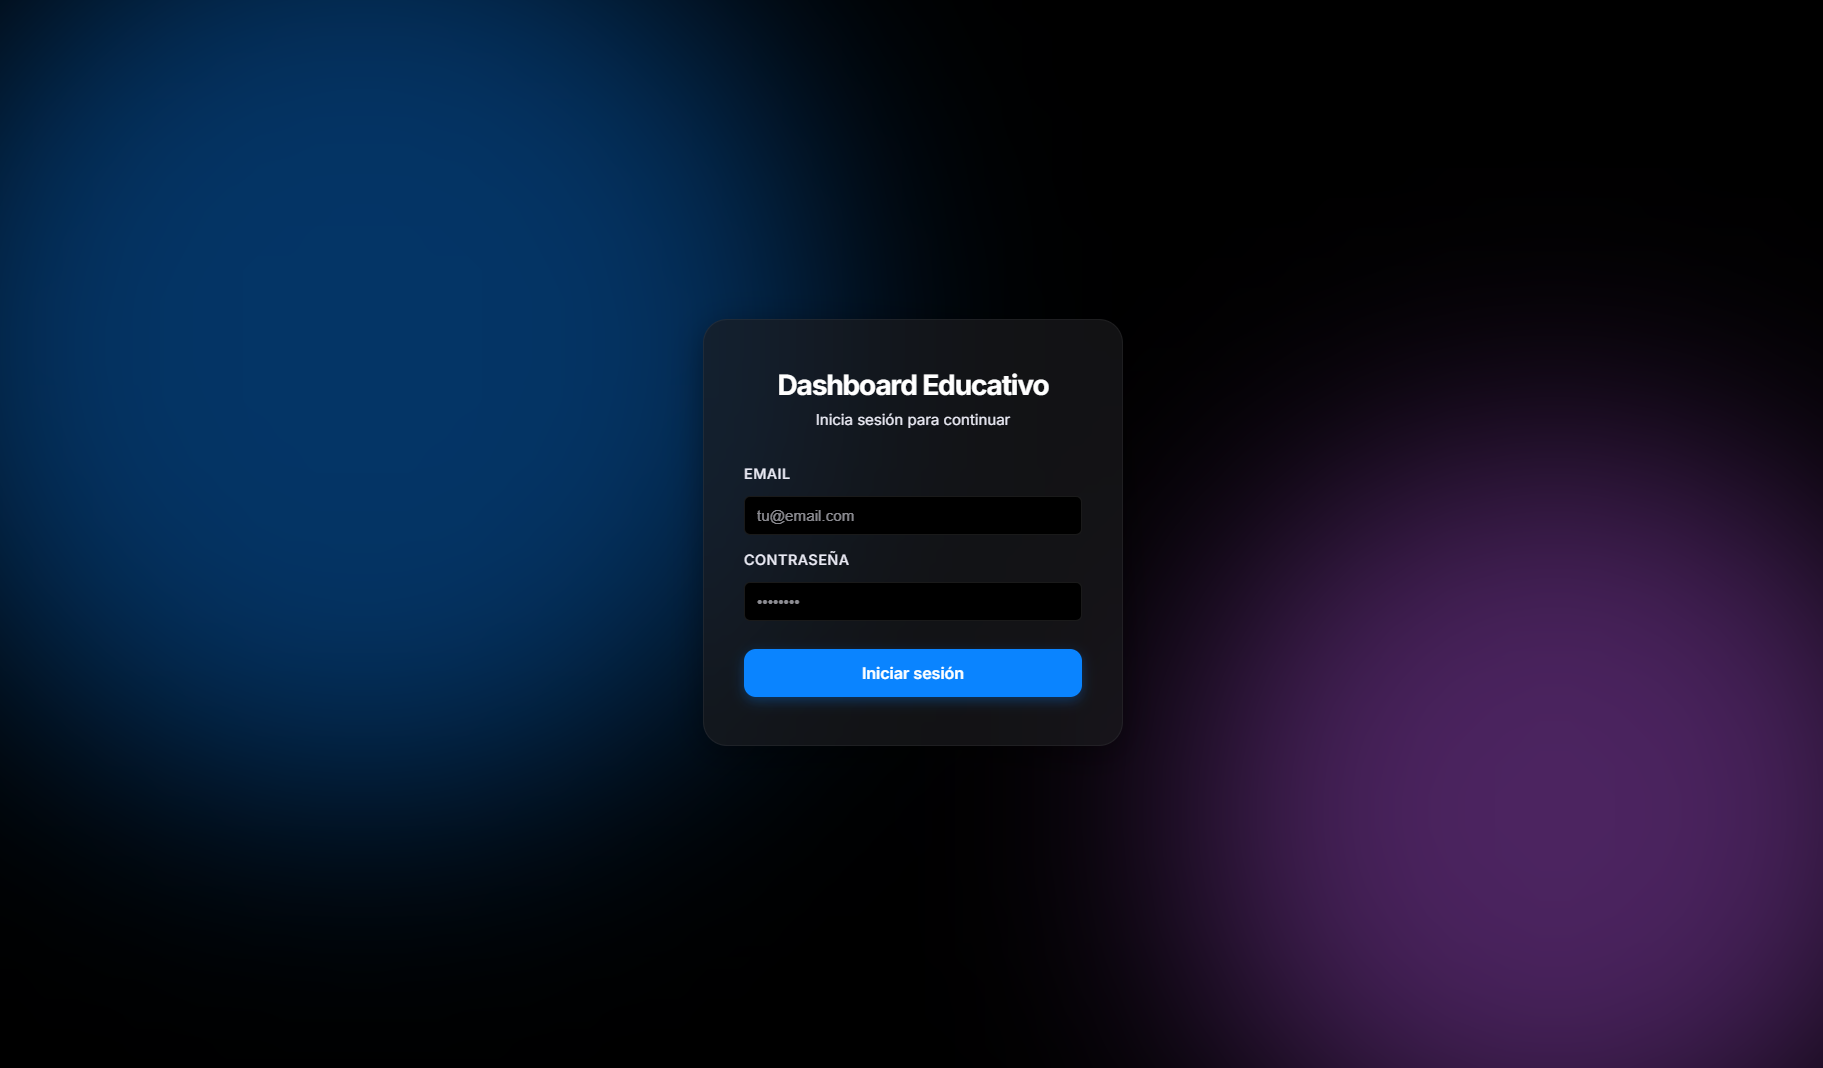
\includegraphics[width=\textwidth]{imaxes/dashboard_login.png}
    \caption{Pantalla de inicio de sesión de la aplicación.}
    \label{fig:dashboard_login}
\end{figure}
% =========================================================================

La \textbf{pantalla de login} solicita únicamente las credenciales de acceso (correo electrónico y contraseña). Tras una autenticación correcta, la aplicación almacena el token de sesión de forma segura y redirige automáticamente al usuario a la vista principal del cuadro de mando. La sesión persiste entre visitas: si el usuario cierra el navegador y lo vuelve a abrir, la aplicación la recupera automáticamente sin necesidad de volver a introducir las credenciales, siempre que el token no haya expirado.

% =========================================================================
\section{Estructura general de la interfaz}
% =========================================================================

Tras el login, el usuario accede a un \textit{layout} de aplicación compuesto por dos áreas diferenciadas: una barra lateral de navegación a la izquierda y el área de contenido principal a la derecha.

\subsection{Barra lateral (Sidebar)}

La barra lateral cumple una doble función: sirve como menú de navegación entre las vistas de la aplicación y alberga los \textbf{filtros globales} que condicionan todos los datos mostrados en pantalla de forma simultánea. Puede contraerse para maximizar el espacio de visualización, mostrando únicamente los iconos de navegación.

Los filtros globales disponibles son cuatro. El \textbf{curso académico} permite seleccionar el año lectivo que se desea analizar; por defecto, la aplicación selecciona automáticamente el curso más reciente disponible en el sistema. El \textbf{tipo de centro} filtra por tipología institucional (IES, CEIP, etc.). El \textbf{centro educativo} permite seleccionar uno o varios centros concretos mediante un selector con búsqueda por nombre, lo que habilita el drilldown desde la vista Macro hacia la Micro. El \textbf{ciclo formativo} restringe el análisis a un ciclo educativo específico. Cualquier cambio en estos filtros se propaga de forma inmediata a todas las visualizaciones activas, sin necesidad de confirmar ni recargar la página. Un botón de \textit{Resetear} restaura los filtros a su estado por defecto.

La barra lateral también incluye un selector de \textbf{tema visual} (modo claro / modo oscuro), que se persiste entre sesiones mediante \textit{localStorage}, y el botón de cierre de sesión. En cuanto a la navegación, el menú ofrece acceso a tres secciones: \textbf{Centro de Mando} (\textit{/macro}), \textbf{Análisis de Centro} (\textit{/micro}), y \textbf{Gestión de Usuarios} (\textit{/users}), esta última visible únicamente para cuentas con rol de administrador.

% =========================================================================
\section{Vista Macro: centro de mando autonómico}

\begin{figure}[htbp]
    \centering
    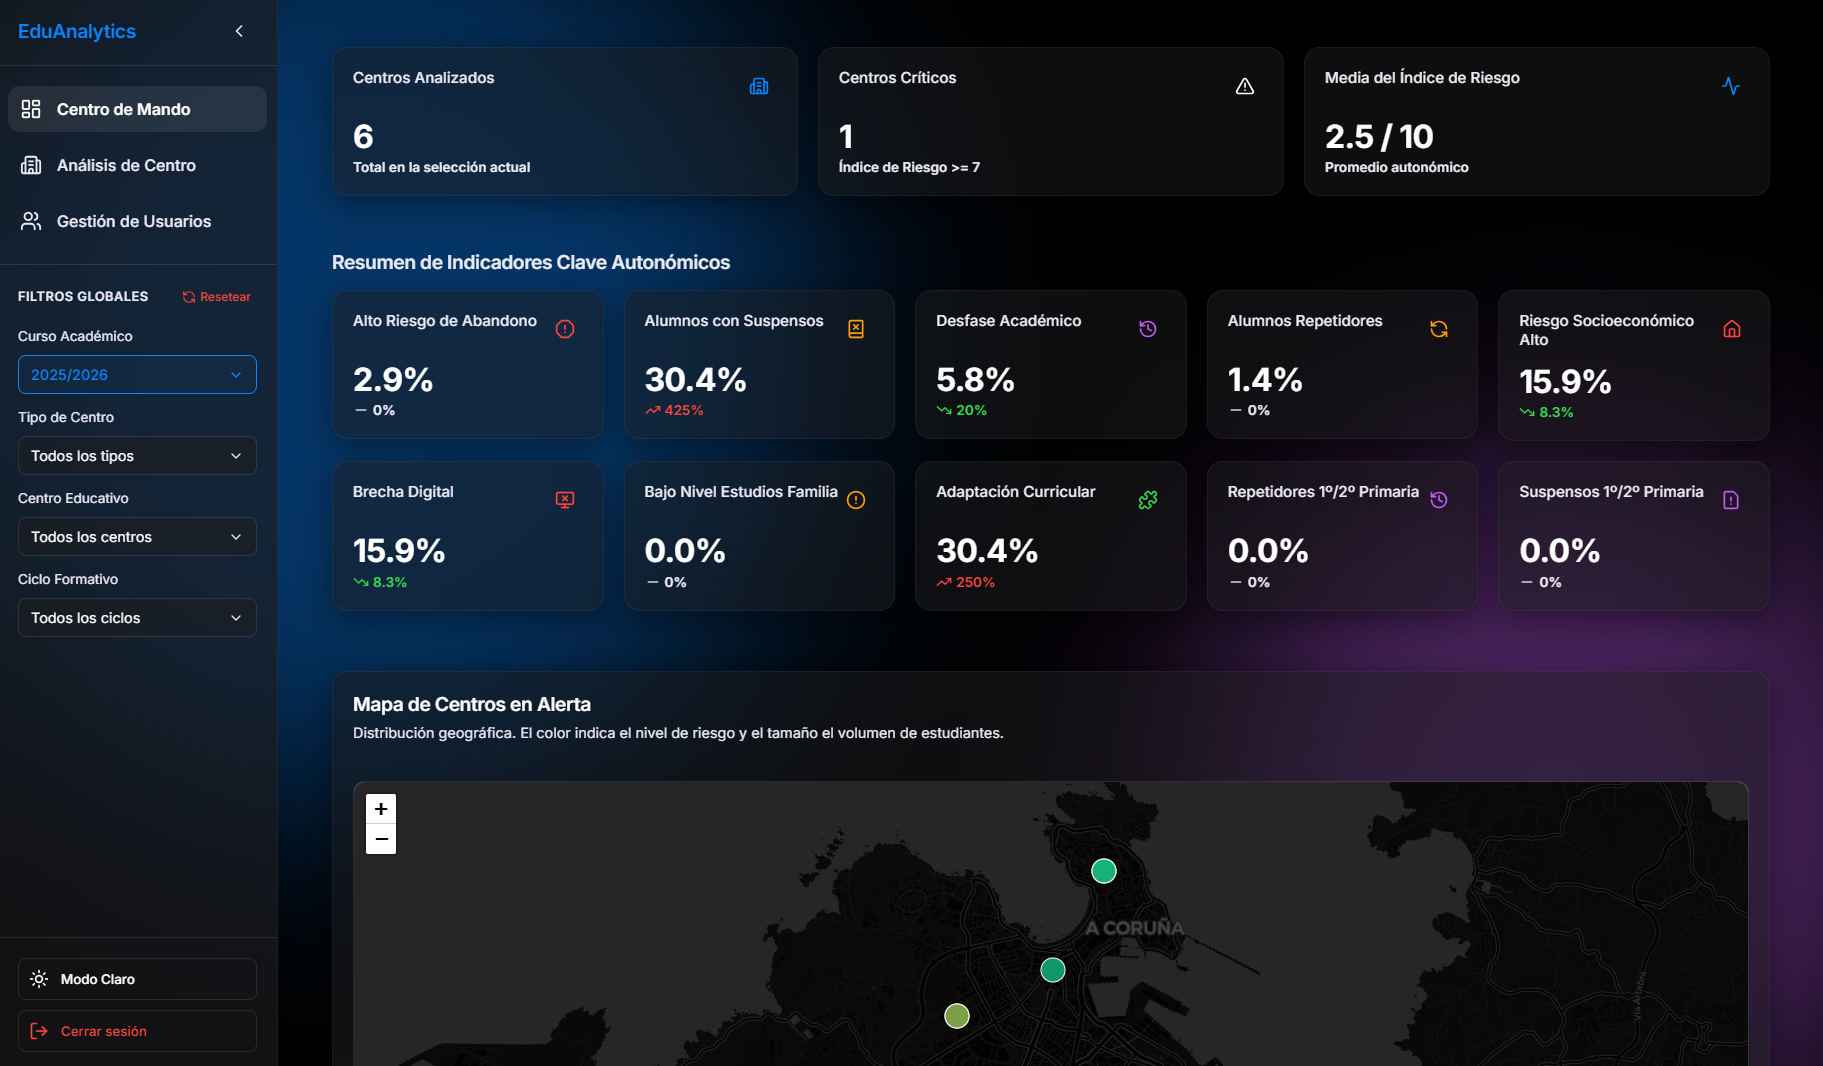
\includegraphics[width=\textwidth]{imaxes/dashboard_cm_1.png}
    \caption{Vista Macro: indicadores autonómicos, alertas institucionales y mapa geográfico.}
    \label{fig:dashboard_cm_1}
\end{figure}
% =========================================================================

La vista \textit{Centro de Mando Autonómico} es el punto de partida habitual del flujo de trabajo. Ofrece una perspectiva agregada del conjunto de centros educativos de la comunidad autónoma, permitiendo al técnico de la administración identificar qué centros concentran mayor riesgo y, por tanto, deben ser priorizados en la asignación de recursos de apoyo, refuerzo o inspección.

\subsection{Indicadores de cabecera}

En la parte superior de la vista se presentan tres \textbf{tarjetas KPI} de resumen que ofrecen una lectura inmediata del estado del sistema: el número total de centros incluidos en la selección activa, el número de centros con índice de riesgo institucional igual o superior a~7 sobre~10 (centros críticos), y la media autonómica del índice de riesgo de todos los centros analizados.

\subsection{Panel de alertas institucionales}

Debajo de los KPI de cabecera, un panel de \textbf{alertas institucionales} desglosa diez métricas de riesgo a escala de centro. Para cada métrica, el indicador muestra el número de centros que superan la mediana autonómica del número de alumnos afectados, calculada a partir de los datos individuales de la vista Micro. Las métricas cubren: alto riesgo de abandono, alumnado con suspensos, desfase académico por edad, repetidores, riesgo socioeconómico alto, brecha digital, bajo nivel de estudios familiar, adaptaciones curriculares, repetidores en 1.º y 2.º de primaria, y suspensos en 1.º y 2.º de primaria.

Estas tarjetas son interactivas: al pulsar sobre cualquiera de ellas, la vista filtra automáticamente el ranking de centros para mostrar únicamente aquellos que superan la mediana en esa métrica concreta, desplazándose de forma suave hasta la sección del ranking. Este mecanismo permite al técnico focalizar la atención en el subconjunto de centros más afectados por un factor de riesgo específico antes de decidir qué tipo de recurso asignar.

\subsection{Mapa geográfico de centros}

Un \textbf{mapa interactivo} muestra la distribución geográfica de todos los centros. Cada centro se representa mediante un marcador circular cuyo color refleja su nivel de riesgo (verde, amarillo o rojo). Al hacer clic sobre un marcador, la aplicación realiza un drilldown automático: fija ese centro en los filtros globales y navega a la vista Micro para mostrar el diagnóstico causal de su índice de riesgo.

\subsection{Gráficos de análisis macro}

\begin{figure}[htbp]
    \centering
    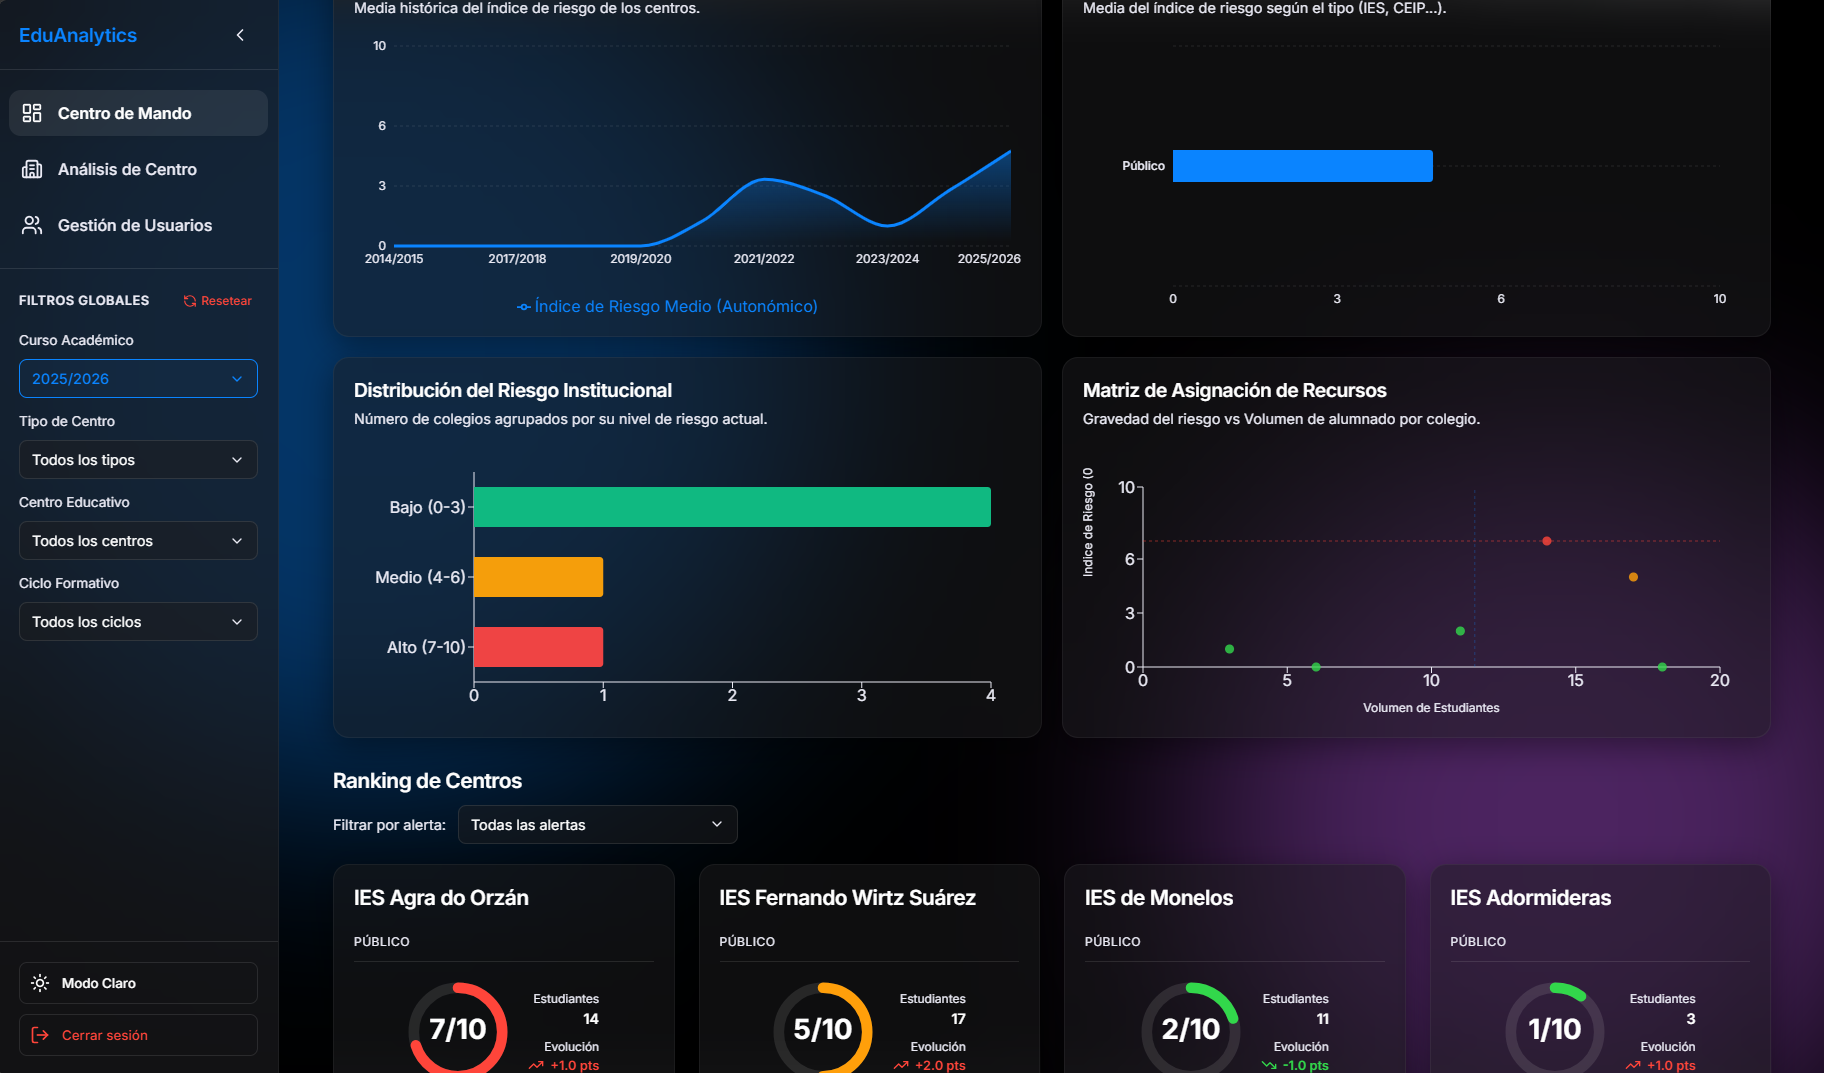
\includegraphics[width=\textwidth]{imaxes/dashboard_cm_2.png}
    \caption{Vista Macro: gráficos de evolución interanual y ranking autonómico de centros.}
    \label{fig:dashboard_cm_2}
\end{figure}

La vista incluye cuatro gráficos complementarios. La \textbf{evolución del riesgo autonómico} es una línea temporal con la media histórica del índice de riesgo de los centros, que permite identificar si la tendencia general mejora o empeora a lo largo de los cursos académicos. La \textbf{comparativa por tipo de centro} es un gráfico de barras que contrasta la media del índice de riesgo según la tipología institucional, revelando si determinados tipos de centro concentran sistemáticamente mayor vulnerabilidad. La \textbf{distribución de riesgo institucional} agrupa los centros en tres niveles (Bajo 0--3, medio 4--6, alto 7--10) mediante barras horizontales; al hacer clic sobre una barra, el ranking inferior se filtra para mostrar únicamente los centros de ese nivel. Por último, la \textbf{matriz de asignación de recursos} es un diagrama de dispersión que enfrenta la gravedad del riesgo (eje horizontal) con el volumen de alumnado (eje vertical) para cada centro, permitiendo identificar visualmente qué centros combinan alto riesgo con gran número de alumnos y, por tanto, representan la mayor prioridad de intervención.

\subsection{Ranking de centros}

En la parte inferior de la vista se muestra el \textbf{ranking completo de centros}, ordenado de mayor a menor índice de riesgo. Cada tarjeta de centro presenta el nombre, el tipo, el número de alumnos, el índice de riesgo con indicador visual de color, y la variación respecto al curso anterior expresada en puntos. Al pulsar sobre una tarjeta, se activa el drilldown hacia la vista Micro con ese centro preseleccionado en los filtros globales.

% =========================================================================
\section{Vista Micro: análisis de centro}

\begin{figure}[htbp]
    \centering
    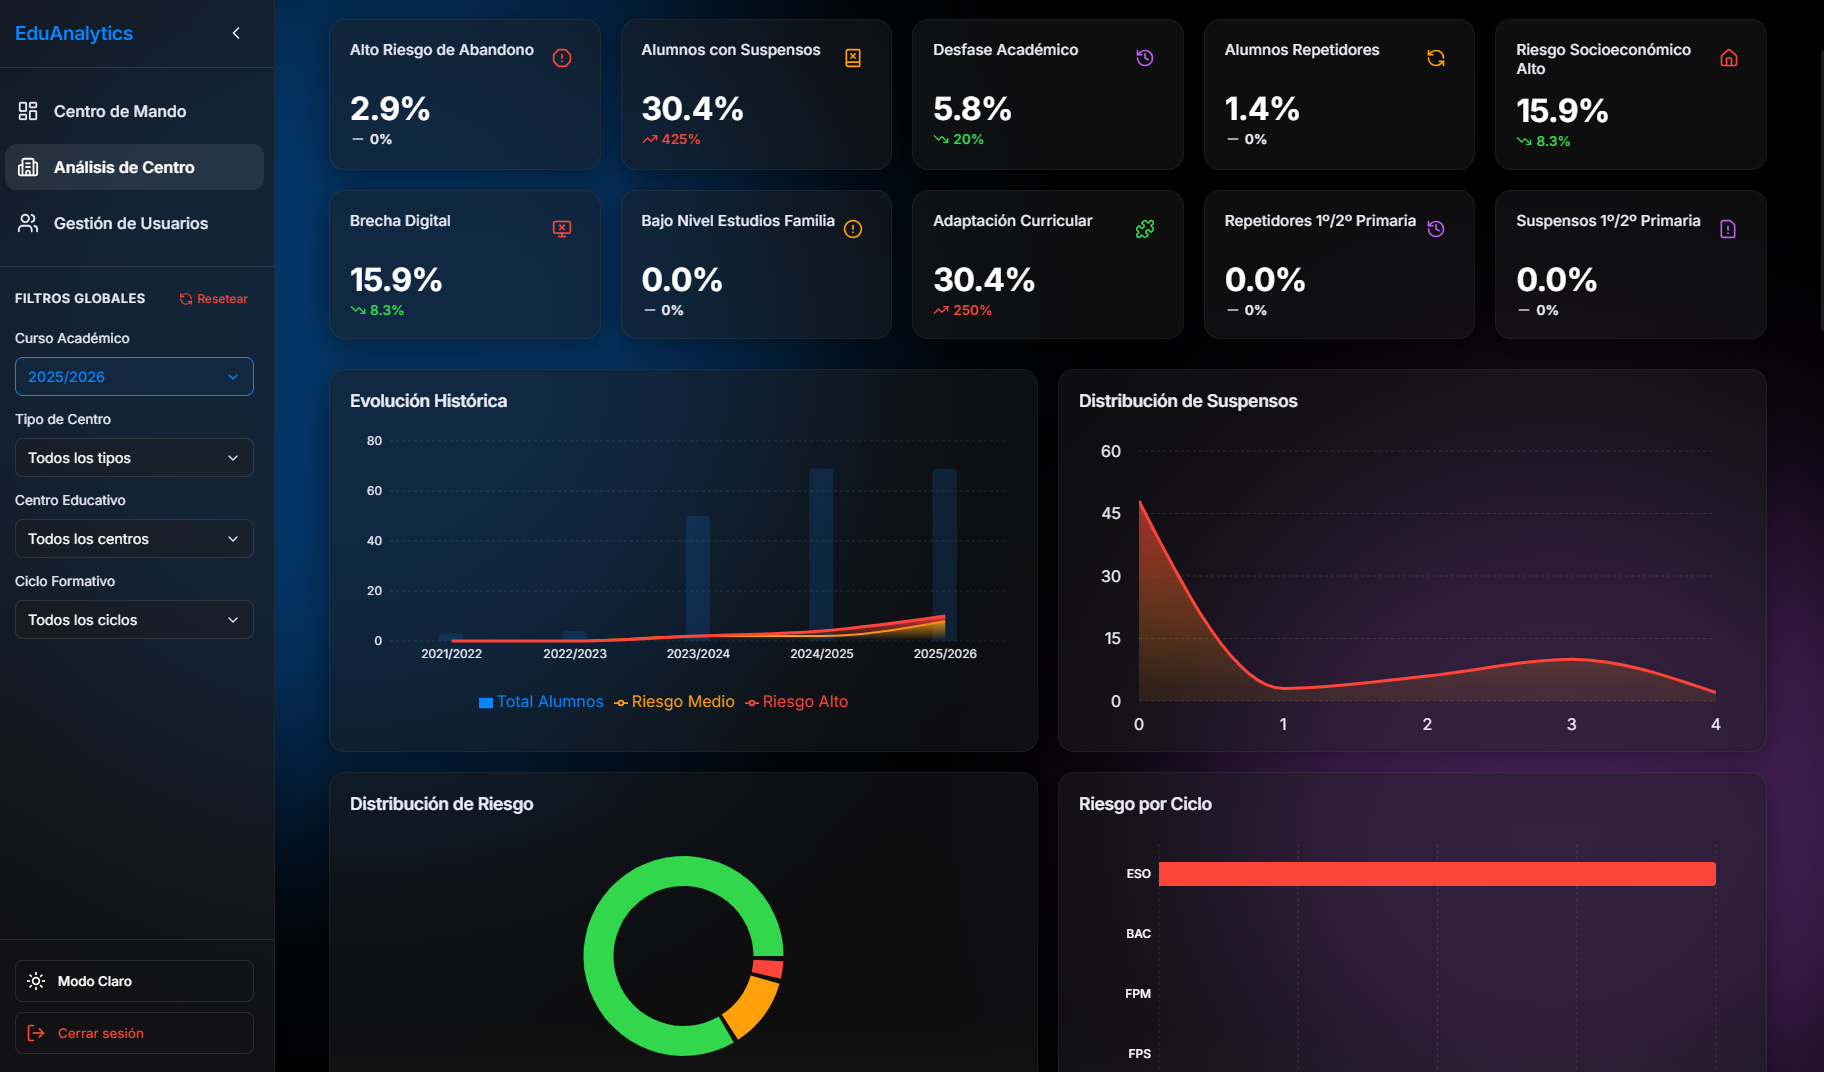
\includegraphics[width=\textwidth]{imaxes/dashboard_ac_1.png}
    \caption{Vista Micro: indicadores de alumnado con comparativa interanual y distribución del riesgo de abandono.}
    \label{fig:dashboard_ac_1}
\end{figure}
% =========================================================================

La vista \textit{Análisis de Centro} es la herramienta de diagnóstico causal del sistema. Se accede a ella bien directamente desde el menú, bien mediante el drilldown desde la vista Macro al seleccionar uno o varios centros concretos. Su propósito es responder a la pregunta de \textit{por qué} un centro presenta el índice de riesgo que tiene, desagregando los factores que lo componen y permitiendo al técnico fundamentar con evidencia la naturaleza de los recursos que deben asignarse.

\subsection{Indicadores de alumnado con comparativa interanual}

La sección superior presenta \textbf{diez tarjetas KPI}, una por cada tipo de alerta, que miden el número de alumnos de los centros seleccionados que presentan ese factor de riesgo en el curso actual (T0), junto con el dato del curso anterior (T-1). Esta comparativa interanual permite evaluar si la situación ha mejorado o empeorado respecto al año precedente, aportando una dimensión temporal al diagnóstico. Las métricas son las mismas diez que en la vista Macro, pero medidas ahora a escala de alumno individual en lugar de a escala de centro.

Cada tarjeta es interactiva: al pulsarla, la tabla de alumnos de la parte inferior se filtra automáticamente para mostrar únicamente los estudiantes que presentan esa alerta, y la vista se desplaza suavemente hasta la tabla. Este mecanismo de \textit{cross-filtering} permite pasar en un solo clic de la lectura del KPI a la lista nominal de alumnos afectados.

\subsection{Gráficos de análisis de alumnado}

\begin{figure}[htbp]
    \centering
    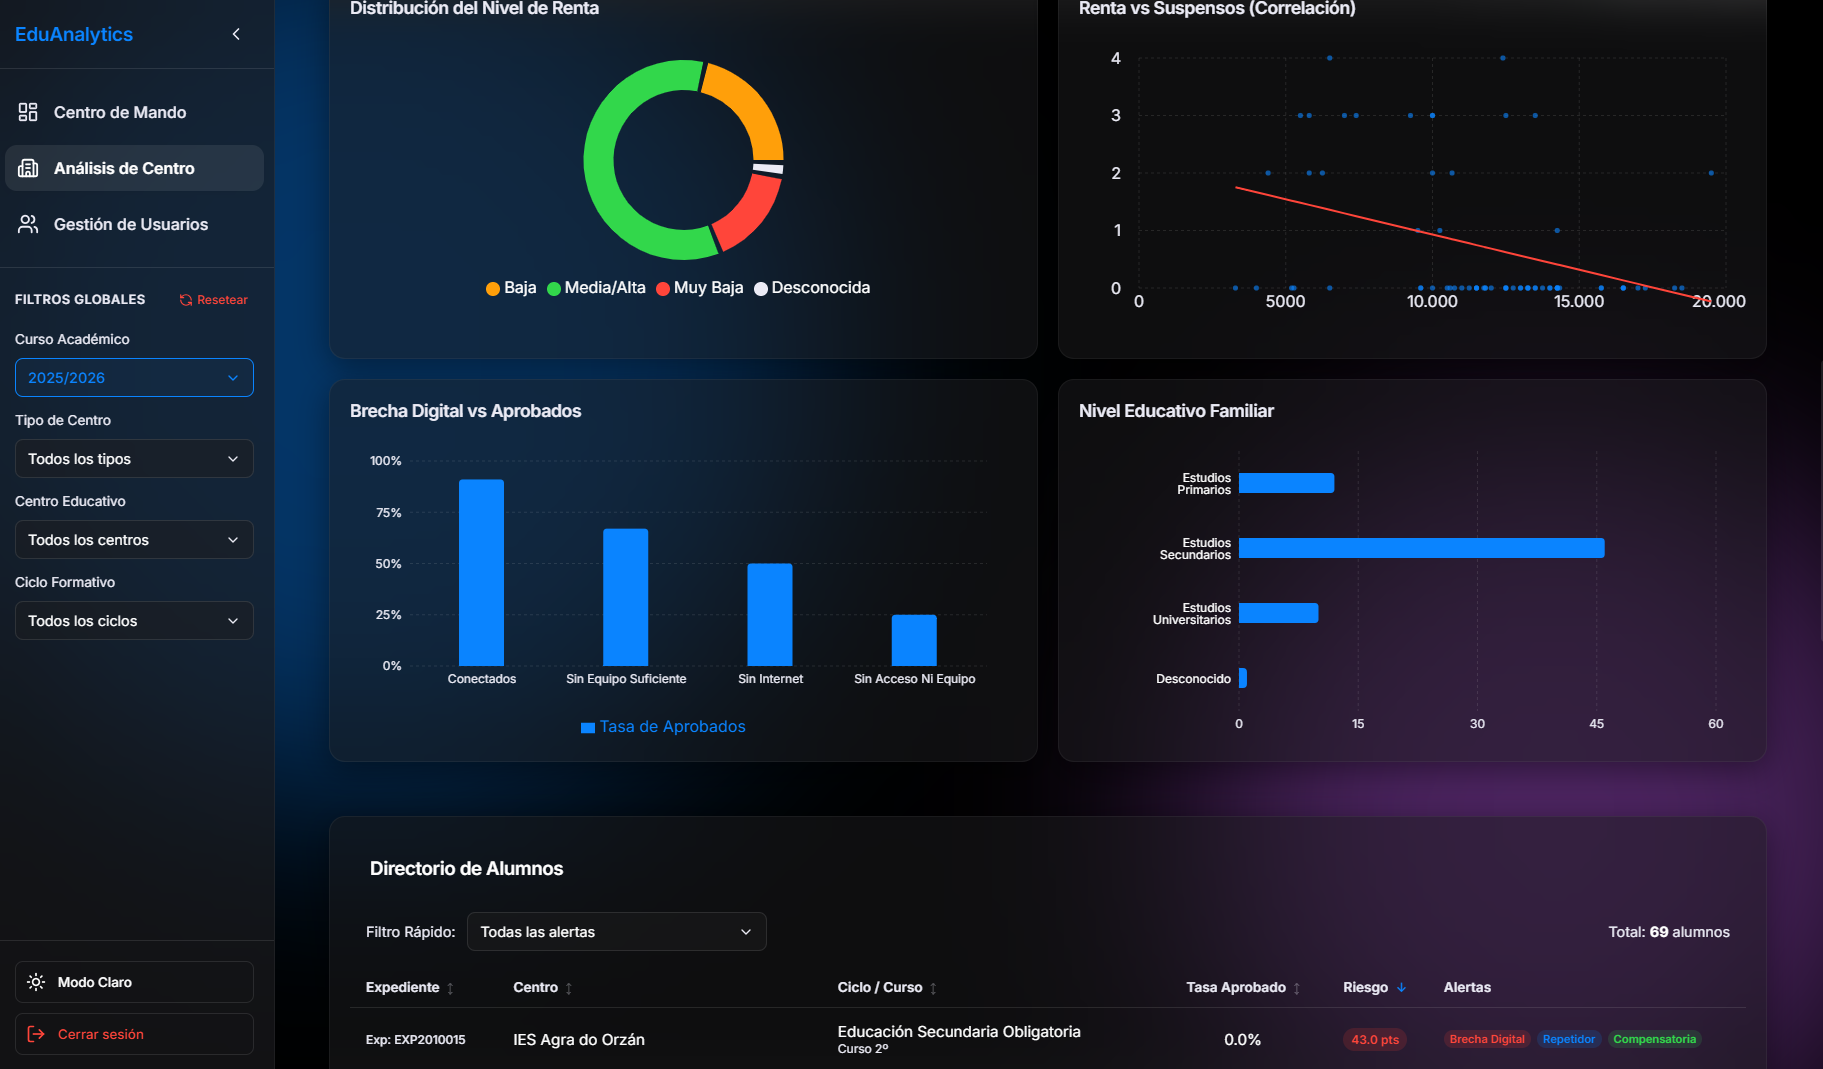
\includegraphics[width=\textwidth]{imaxes/dashboard_ac_2.png}
    \caption{Vista Micro: gráficos de factores socioeconómicos (renta, brecha digital, nivel educativo familiar) y correlaciones.}
    \label{fig:dashboard_ac_2}
\end{figure}

Ocho gráficos ofrecen distintas perspectivas sobre la composición del riesgo en los centros seleccionados. La \textbf{evolución histórica} muestra la tendencia del riesgo medio de abandono en los últimos cinco cursos académicos. La \textbf{distribución de suspensos} es un histograma que muestra cuántos alumnos acumulan 0, 1, 2, 3 o más asignaturas suspensas. La \textbf{distribución de riesgo} es un gráfico circular que clasifica al alumnado en los tres niveles de riesgo (Bajo, medio, alto). El \textbf{riesgo por ciclo} compara el porcentaje de alumnado en riesgo crítico desglosado por ciclo educativo, revelando en qué etapas se concentra el problema.

Los cuatro gráficos restantes analizan los factores socioeconómicos y familiares: la \textbf{distribución del nivel de renta} muestra la proporción de familias en cada tramo (Muy baja, baja, media/alta); el gráfico de \textbf{renta frente a suspensos} es un diagrama de dispersión que evidencia la correlación entre vulnerabilidad económica y rendimiento académico; el gráfico de \textbf{brecha digital frente a aprobados} relaciona el acceso a dispositivos e internet con la tasa de aprobado; y el gráfico de \textbf{nivel educativo familiar} muestra la distribución del máximo nivel de estudios alcanzado por los progenitores. Estos cuatro indicadores son especialmente relevantes para determinar si los recursos que necesita un centro son de naturaleza académica (refuerzo curricular) o socioeconómica (becas, dotación tecnológica, programas de acompañamiento familiar).

\subsection{Directorio de alumnos}

En la parte inferior de la vista se encuentra el \textbf{Directorio de Alumnos}, una tabla paginada (25 registros por página) que lista a todos los estudiantes que cumplen los filtros activos. Para cada alumno se muestra el número de expediente, el centro educativo y ciclo al que pertenece, la tasa de aprobado, la puntuación de riesgo de abandono con indicador visual de nivel (Bajo, medio o alto), y los \textit{badges} de alertas activas (Brecha digital, renta baja, repetidor, discapacidad o compensatoria).

La tabla permite ordenación interactiva por cualquiera de sus columnas, tanto ascendente como descendente, e incorpora un filtro rápido multicriterio por tipo de alerta que puede combinarse con los filtros globales del sidebar. Un contador en tiempo real informa del total de alumnos que coinciden con la selección activa.

% =========================================================================
\section{Gestión de usuarios}
% =========================================================================

La sección de \textbf{Gestión de Usuarios} es accesible únicamente para cuentas con rol de administrador. Permite mantener el directorio de cuentas de acceso a la aplicación mediante las operaciones habituales de creación, edición y eliminación de usuarios. El sistema aplica reglas de protección sobre la cuenta del superadministrador (identificador~1): no puede ser eliminada, degradada a rol de visualizador ni modificada por otros administradores, garantizando que siempre exista al menos una cuenta con acceso completo al sistema.

% =========================================================================
\section{Casos de uso principales}
% =========================================================================

A continuación se describen los flujos de trabajo más representativos que ilustran cómo la herramienta apoya el proceso de toma de decisiones en la distribución de recursos educativos.

\subsection{Caso de uso 1: priorización de centros para asignación de recursos de apoyo}

Un técnico de la administración educativa autonómica accede a la vista \textit{Centro de Mando} al inicio del curso académico. Selecciona el curso en el filtro del sidebar y observa que la media del índice de riesgo autonómico ha subido 0,4 puntos respecto al curso anterior y que hay tres centros con índice crítico ($\geq 7$). Pulsa sobre la tarjeta de alerta \textit{Repetidores 1.º/2.º de primaria} para filtrar el ranking por esa métrica. Identifica dos centros CEIP que concentran la mayor proporción de alumnos repetidores en ciclos iniciales. Hace clic sobre la tarjeta de uno de ellos para realizar el drilldown hacia la vista Micro.

En la vista Micro, con ese centro preseleccionado, el técnico observa que el KPI de \textit{Bajo nivel de estudios familiar} es el más elevado y que el gráfico de \textit{Nivel educativo familiar} confirma que más del 60\% de las familias no ha completado la educación secundaria. Con esta evidencia, concluye que el recurso adecuado no es refuerzo curricular sino un programa de acompañamiento familiar, y fundamenta así su propuesta de asignación ante el órgano competente.

\subsection{Caso de uso 2: diagnóstico de la brecha digital en centros de zona rural}

El técnico filtra la vista Macro por tipo de centro CEIP y observa en el mapa que varios centros de zonas rurales presentan marcadores rojos. Selecciona el conjunto de esos centros mediante el filtro de centro educativo y navega a la vista Micro. El KPI de \textit{Brecha digital} muestra un número significativamente superior al de la media autonómica, y el gráfico de \textit{Brecha digital frente a aprobados} evidencia una correlación negativa clara entre la falta de dispositivos en el hogar y la tasa de aprobado. Esta información sirve de base para solicitar la dotación de equipos informáticos y conectividad en el marco de un programa de reducción de la brecha digital.

\subsection{Caso de uso 3: evaluación del impacto de una intervención previa}

Un inspector de educación desea evaluar el impacto de un programa de refuerzo implantado hace dos cursos en un conjunto de centros de una comarca. Selecciona esos centros en el filtro de centro educativo y consulta el gráfico de \textbf{evolución del riesgo autonómico} en la vista Macro. La línea temporal muestra una reducción sostenida del índice de riesgo medio en los dos últimos cursos para esa selección. A continuación, realiza el drilldown a la vista Micro y comprueba que el KPI de \textit{Alumnado con suspensos} ha descendido en T0 respecto a T-1, mientras que el de \textit{Alto riesgo de abandono} se mantiene estable. Esta lectura combinada permite concluir que el programa ha tenido efecto sobre el rendimiento académico inmediato pero que persisten factores estructurales de riesgo que requieren intervenciones adicionales de carácter socioeconómico.

\subsection{Caso de uso 4: análisis comparativo por tipo de centro}

Un técnico de planificación educativa necesita determinar si los centros de Formación Profesional presentan un perfil de riesgo diferenciado respecto a los institutos de educación secundaria. Filtra la vista Macro por tipo de centro y alterna entre IES y ciclos de FP, comparando el gráfico de \textit{Comparativa por Tipo de Centro} y la distribución de alertas en el panel institucional. Observa que los centros de FP concentran una mayor proporción de alumnado con desfase académico por edad y con riesgo socioeconómico alto, lo que orienta la planificación de recursos específicos para ese tipo de centro en el presupuesto del siguiente ejercicio.
